\documentclass[11pt,a4paper]{article}
\usepackage[margin=2cm]{geometry}
\usepackage{graphicx}
\usepackage{xcolor}
\usepackage{tcolorbox}
\usepackage{enumitem}
\usepackage{fancyhdr}
\usepackage{tikz}
\usepackage{tabularx}
\usepackage{booktabs}
\usepackage{multicol}
\usepackage{amssymb}
\setlength{\headheight}{14pt}

% ============================================================
% DIAMOND COLOR SCHEME
% ============================================================
\definecolor{challenge}{RGB}{148,103,189}
\definecolor{explore}{RGB}{52,152,219}
\definecolor{generate}{RGB}{46,204,113}
\definecolor{peak}{RGB}{241,196,15}
\definecolor{filter}{RGB}{230,126,34}
\definecolor{refine}{RGB}{231,76,60}
\definecolor{strategy}{RGB}{192,57,43}
\definecolor{mlpurple}{RGB}{51,51,178}
\definecolor{mllavender}{RGB}{173,173,224}
\definecolor{mllavender2}{RGB}{193,193,232}
\definecolor{promptbg}{RGB}{240,248,255}

% ============================================================
% CUSTOM BOXES
% ============================================================
\tcbset{
    promptbox/.style={
        colback=promptbg,
        colframe=mlpurple,
        boxrule=1pt,
        arc=3pt,
        left=8pt,
        right=8pt,
        top=6pt,
        bottom=6pt,
        fonttitle=\bfseries\small,
        title=LLM Prompt (copy and paste)
    },
    writebox/.style={
        colback=white,
        colframe=mllavender,
        boxrule=0.5pt,
        arc=2pt,
        left=4pt,
        right=4pt,
        top=4pt,
        bottom=4pt
    },
    phasebox/.style={
        colback=#1!10,
        colframe=#1,
        boxrule=2pt,
        arc=4pt,
        fonttitle=\bfseries\large,
        coltitle=white,
        colbacktitle=#1
    }
}

% ============================================================
% HEADER/FOOTER
% ============================================================
\pagestyle{fancy}
\fancyhf{}
\renewcommand{\headrulewidth}{0.4pt}
\fancyhead[L]{\textcolor{mlpurple}{\textbf{Innovation Diamond Worksheet}}}
\fancyhead[R]{\textcolor{mllavender}{1 $\rightarrow$ 5,000 $\rightarrow$ 5}}
\fancyfoot[C]{\thepage}

% ============================================================
% DOCUMENT
% ============================================================
\begin{document}

\begin{center}
{\Huge\textbf{\textcolor{mlpurple}{Innovation Diamond}}}\\[0.3em]
{\Large\textcolor{mllavender}{Student Worksheet}}\\[0.5em]
{\large Apply the 1 $\rightarrow$ 5,000 $\rightarrow$ 5 Framework to Your Own Challenge}
\end{center}

\vspace{0.5cm}

\noindent\textbf{Name:} \underline{\hspace{6cm}} \hfill \textbf{Date:} \underline{\hspace{4cm}}

\vspace{1cm}

% ============================================================
% PAGE 1: DEFINE YOUR CHALLENGE
% ============================================================
\begin{tcolorbox}[phasebox=challenge, title={\textcolor{white}{Page 1: Define Your Challenge (1)}}]

\textbf{Your Innovation Challenge} (write in 1-2 sentences):
\begin{tcolorbox}[writebox, height=2.5cm]
\vspace{2cm}
\end{tcolorbox}

\vspace{0.3cm}

\textbf{Key Stakeholders} (who is affected?):
\begin{enumerate}[itemsep=0.3cm]
\item \underline{\hspace{10cm}}
\item \underline{\hspace{10cm}}
\item \underline{\hspace{10cm}}
\item \underline{\hspace{10cm}}
\item \underline{\hspace{10cm}}
\end{enumerate}

\textbf{Constraints} (check all that apply):
\begin{itemize}[itemsep=0.1cm]
\item[$\square$] Budget limitations
\item[$\square$] Time constraints
\item[$\square$] Technical feasibility
\item[$\square$] Regulatory/compliance
\item[$\square$] Resource availability
\item[$\square$] Other: \underline{\hspace{5cm}}
\end{itemize}

\textbf{Success Criteria} (how will you know it worked?):
\begin{enumerate}[itemsep=0.3cm]
\item \underline{\hspace{12cm}}
\item \underline{\hspace{12cm}}
\item \underline{\hspace{12cm}}
\end{enumerate}

\end{tcolorbox}

\begin{tcolorbox}[promptbox]
\small\texttt{Help me refine this innovation challenge: [paste your challenge]. Identify 5 key stakeholders, potential constraints, and 3 measurable success criteria. Format as bullet points.}
\end{tcolorbox}

\newpage

% ============================================================
% PAGE 2: DIVERGENT PHASE
% ============================================================
\begin{tcolorbox}[phasebox=generate, title={\textcolor{white}{Page 2: Divergent Phase (1 $\rightarrow$ 1,000)}}]

\textbf{10 Dimensions to Explore} (different angles to approach your challenge):

\begin{tabularx}{\textwidth}{|c|X|c|X|}
\hline
1 & \hspace{4cm} & 6 & \hspace{4cm} \\[0.5cm]
\hline
2 & & 7 & \\[0.5cm]
\hline
3 & & 8 & \\[0.5cm]
\hline
4 & & 9 & \\[0.5cm]
\hline
5 & & 10 & \\[0.5cm]
\hline
\end{tabularx}

\vspace{0.5cm}

\textbf{Initial Ideas} (aim for 20-50, continue on separate paper):

\begin{tcolorbox}[writebox, height=7cm]
\begin{multicols}{2}
\begin{enumerate}[itemsep=0.25cm]
\item
\item
\item
\item
\item
\item
\item
\item
\item
\item
\item
\item
\item
\item
\item
\item
\item
\item
\item
\item
\end{enumerate}
\end{multicols}
\end{tcolorbox}

\end{tcolorbox}

\begin{tcolorbox}[promptbox]
\small\texttt{Given this innovation challenge: [challenge], generate 50 diverse solution approaches across these dimensions: [list your 10 dimensions]. Include unconventional and creative ideas. Number each idea.}
\end{tcolorbox}

\newpage

% ============================================================
% PAGE 3: PEAK EXPLORATION
% ============================================================
\begin{tcolorbox}[phasebox=peak, title={\textcolor{white}{Page 3: Peak Exploration (1,000 $\rightarrow$ 5,000)}}]

\textbf{Idea Combinations} (mix ideas from different dimensions):

\begin{tabularx}{\textwidth}{|X|X|X|}
\hline
\textbf{Idea A} & \textbf{+ Idea B} & \textbf{= Hybrid Solution} \\
\hline
& & \\[0.8cm]
\hline
& & \\[0.8cm]
\hline
& & \\[0.8cm]
\hline
& & \\[0.8cm]
\hline
& & \\[0.8cm]
\hline
\end{tabularx}

\vspace{0.5cm}

\textbf{Theme Clusters} (group similar ideas into 5 themes):

\begin{tabularx}{\textwidth}{|X|X|}
\hline
\textbf{Theme 1:} \underline{\hspace{3cm}} & \textbf{Theme 2:} \underline{\hspace{3cm}} \\
Ideas: & Ideas: \\[2cm]
\hline
\textbf{Theme 3:} \underline{\hspace{3cm}} & \textbf{Theme 4:} \underline{\hspace{3cm}} \\
Ideas: & Ideas: \\[2cm]
\hline
\multicolumn{2}{|c|}{\textbf{Theme 5:} \underline{\hspace{3cm}}} \\
\multicolumn{2}{|c|}{Ideas:} \\[1.5cm]
\hline
\end{tabularx}

\end{tcolorbox}

\begin{tcolorbox}[promptbox]
\small\texttt{Take these 50 ideas [paste list] and: 1) Identify 5 major themes, 2) Create 10 hybrid solutions by combining ideas from different themes, 3) For each hybrid, explain why the combination creates value.}
\end{tcolorbox}

\newpage

% ============================================================
% PAGE 4: CONVERGENT PHASE
% ============================================================
\begin{tcolorbox}[phasebox=filter, title={\textcolor{white}{Page 4: Convergent Phase (5,000 $\rightarrow$ 50)}}]

\textbf{Feasibility vs Impact Matrix} (place your top ideas):

\begin{center}
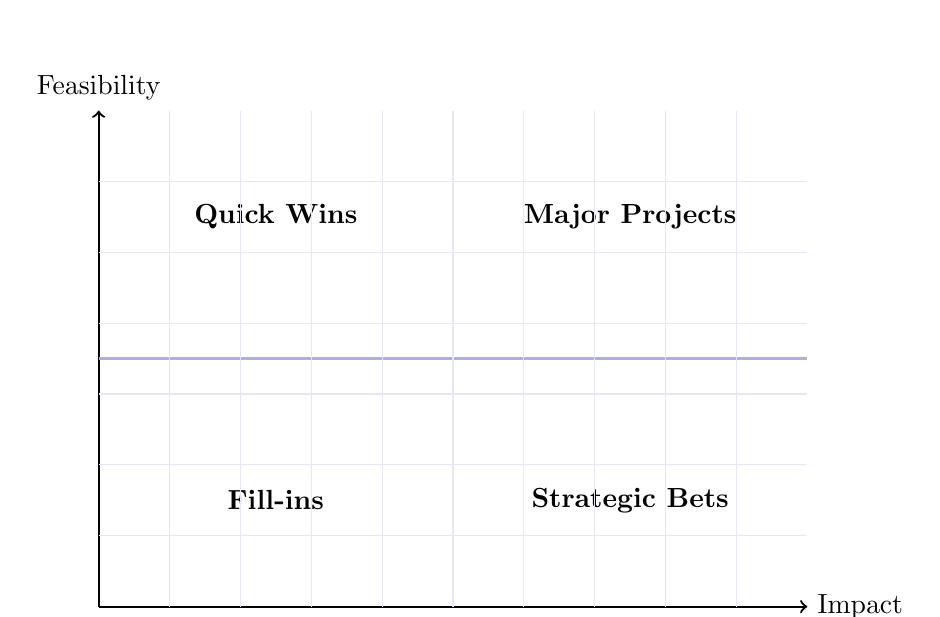
\begin{tikzpicture}[scale=0.9]
\draw[thick,->] (0,0) -- (10,0) node[right] {Impact};
\draw[thick,->] (0,0) -- (0,7) node[above] {Feasibility};
\draw[mllavender, thick] (5,0) -- (5,7);
\draw[mllavender, thick] (0,3.5) -- (10,3.5);
\node at (2.5,5.5) {\textbf{Quick Wins}};
\node at (7.5,5.5) {\textbf{Major Projects}};
\node at (2.5,1.5) {\textbf{Fill-ins}};
\node at (7.5,1.5) {\textbf{Strategic Bets}};
% Grid for plotting
\foreach \x in {1,2,...,9} \draw[mllavender!30] (\x,0) -- (\x,7);
\foreach \y in {1,2,...,6} \draw[mllavender!30] (0,\y) -- (10,\y);
\end{tikzpicture}
\end{center}

\vspace{0.3cm}

\textbf{Top 10 Ideas} (score each 1-5):

\begin{tabularx}{\textwidth}{|c|X|c|c|c|}
\hline
\textbf{\#} & \textbf{Idea Description} & \textbf{Feasibility} & \textbf{Impact} & \textbf{Total} \\
\hline
1 & & /5 & /5 & /10 \\
\hline
2 & & /5 & /5 & /10 \\
\hline
3 & & /5 & /5 & /10 \\
\hline
4 & & /5 & /5 & /10 \\
\hline
5 & & /5 & /5 & /10 \\
\hline
6 & & /5 & /5 & /10 \\
\hline
7 & & /5 & /5 & /10 \\
\hline
8 & & /5 & /5 & /10 \\
\hline
9 & & /5 & /5 & /10 \\
\hline
10 & & /5 & /5 & /10 \\
\hline
\end{tabularx}

\end{tcolorbox}

\begin{tcolorbox}[promptbox]
\small\texttt{Evaluate these ideas [paste top 20] on: Feasibility (1-5, where 5=easy to implement) and Impact (1-5, where 5=high value). Return a ranked table with scores and brief justification for each.}
\end{tcolorbox}

\newpage

% ============================================================
% PAGE 5: FINAL STRATEGIES
% ============================================================
\begin{tcolorbox}[phasebox=strategy, title={\textcolor{white}{Page 5: Final Strategies (50 $\rightarrow$ 5)}}]

\textbf{Your 5 Strategic Solutions}:

\begin{tcolorbox}[writebox]
\textbf{Strategy 1:} \underline{\hspace{8cm}}\\[0.3cm]
Description: \hrulefill\\[0.3cm]
Key Actions: 1) \underline{\hspace{4cm}} 2) \underline{\hspace{4cm}} 3) \underline{\hspace{4cm}}
\end{tcolorbox}

\begin{tcolorbox}[writebox]
\textbf{Strategy 2:} \underline{\hspace{8cm}}\\[0.3cm]
Description: \hrulefill\\[0.3cm]
Key Actions: 1) \underline{\hspace{4cm}} 2) \underline{\hspace{4cm}} 3) \underline{\hspace{4cm}}
\end{tcolorbox}

\begin{tcolorbox}[writebox]
\textbf{Strategy 3:} \underline{\hspace{8cm}}\\[0.3cm]
Description: \hrulefill\\[0.3cm]
Key Actions: 1) \underline{\hspace{4cm}} 2) \underline{\hspace{4cm}} 3) \underline{\hspace{4cm}}
\end{tcolorbox}

\begin{tcolorbox}[writebox]
\textbf{Strategy 4:} \underline{\hspace{8cm}}\\[0.3cm]
Description: \hrulefill\\[0.3cm]
Key Actions: 1) \underline{\hspace{4cm}} 2) \underline{\hspace{4cm}} 3) \underline{\hspace{4cm}}
\end{tcolorbox}

\begin{tcolorbox}[writebox]
\textbf{Strategy 5:} \underline{\hspace{8cm}}\\[0.3cm]
Description: \hrulefill\\[0.3cm]
Key Actions: 1) \underline{\hspace{4cm}} 2) \underline{\hspace{4cm}} 3) \underline{\hspace{4cm}}
\end{tcolorbox}

\textbf{30-Day Quick Start} (first action for each):
\begin{enumerate}[itemsep=0.2cm]
\item Strategy 1: \underline{\hspace{10cm}}
\item Strategy 2: \underline{\hspace{10cm}}
\item Strategy 3: \underline{\hspace{10cm}}
\item Strategy 4: \underline{\hspace{10cm}}
\item Strategy 5: \underline{\hspace{10cm}}
\end{enumerate}

\end{tcolorbox}

\begin{tcolorbox}[promptbox]
\small\texttt{From these top 10 scored ideas [paste], select 5 final strategies. For each: 1) Give it a memorable name, 2) Write a 2-sentence description, 3) List 3 concrete next actions, 4) Identify the main risk and mitigation.}
\end{tcolorbox}

\end{document}
